\documentclass{article}
\usepackage{graphicx} % Required for the \includegraphics command

\begin{document}

\section{About the Data}
The data is pulled from IPUMS, downloaded as a CSV. We chose the variables City, City Population, and OCC1950, which are the census occupation codes from 1950.

\subsection{Data Cleaning}
\begin{enumerate}
    \item Remove rows that have 0 in "CITYPOP". A city would not have 0 population, so it is likely that this information is simply missing. 0 values account for very little of our data set.
    \item Group by "CITY" and count how many distinct entries there are in "OCC1950" per city, put this result in a new column named OCCCOUNT. We use 1950 census codes because these codes are available across many datasets, and allow for easier comparison.
    \item Now that we have a count of how many occupations appear in each city, we can remove rows where there are duplicates in the "CITY" column. This leaves us with one entry per city with the occupation count.
    \item Create a plot with City Population on the X-axis and Occupation Count on the Y-Axis.
\end{enumerate}

\subsection{Plots}
\begin{figure}[h]
    \centering
    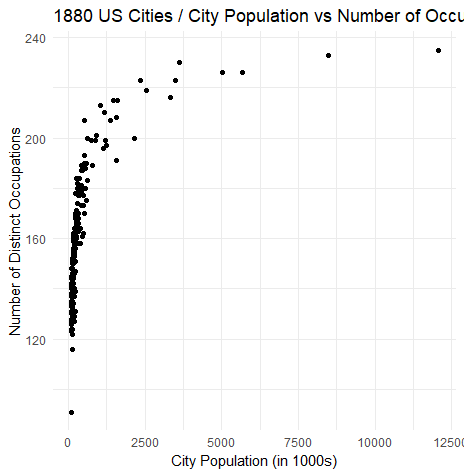
\includegraphics[width=0.4\textwidth]{PS6a_Glass.png}
    \caption{Plot of PS6a Glass: Here we have a look at 1880 census data. It shows a non-linear relationship between the amount of unique occupations in a city and a city's population.}
    \label{fig:PS6a_Glass}
\end{figure}

\begin{figure}[h]
    \centering
    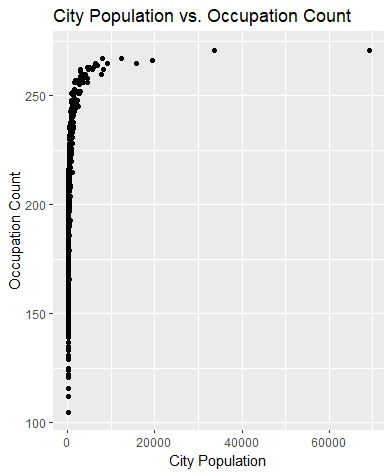
\includegraphics[width=0.4\textwidth]{PS6b_Glass.png}
    \caption{Plot of PS6b Glass: Here we have a look at 1930 census data. It shows a non-linear relationship between the amount of unique occupations in a city and a city's population.}
    \label{fig:PS6b_Glass}
\end{figure}

\begin{figure}[h]
    \centering
    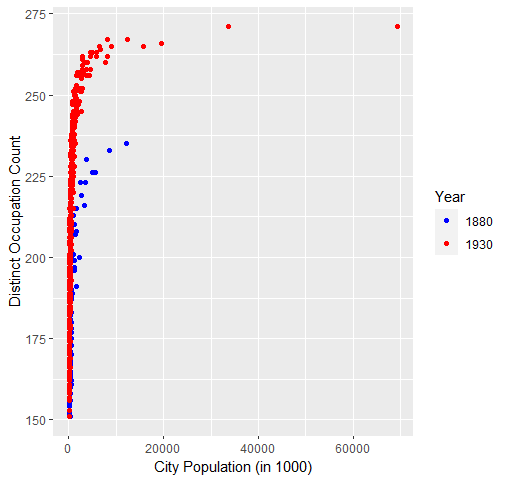
\includegraphics[width=0.4\textwidth]{PS6c_Glass.png}
    \caption{Plot of PS6c Glass: This plot shows both datasets overlaid for better comparison of occupation growth and population.}
    \label{fig:PS6c_Glass}
\end{figure}

\end{document}

